\documentclass[10pt]{article}\usepackage[margin=18mm]{geometry}\usepackage{graphicx}\setlength{\parskip}{5pt}\setlength{\parindent}{0pt}\title{Stage VI-0.2: Hierarchical World Model v2}\author{Frozen-data offline smoke validation}\date{2026-07-12}\begin{document}\maketitle\section{Decision}Decision D - insufficient frozen artifacts is the single main decision.\section{Artifact gate}The 131-field frozen exact schema contains no fixed-k spectrum, eigenvalue curve, DOS proxy, spectral-minimum count, or spectral curvature. Free-energy basin metadata were not misused as spectral fingerprints.\section{Executed smoke}Levels 1, 2, and 4 were revalidated. Level 3 compares the old log-gap/k-gap output with a log-gap-only ablation. Within-run, cross-run, calibration, risk-coverage, probe, replay, and reconstruction tests were completed.\section{Numerical summary}Mean spatial SC AUROC is 0.977. Median spatial $R^2$ is 0.432 (Level 1), 0.799 (Level 2), 0.086 (log-gap-only Level 3), and 0.908 (Level 4). No run/level replay uncertainty trajectory is monotonic.\section{Conclusion}The log-gap-only ablation is not a replacement spectral fingerprint. Full-local and EIG are blocked. No learned state is transferable.\clearpage\begin{figure}[p]\centering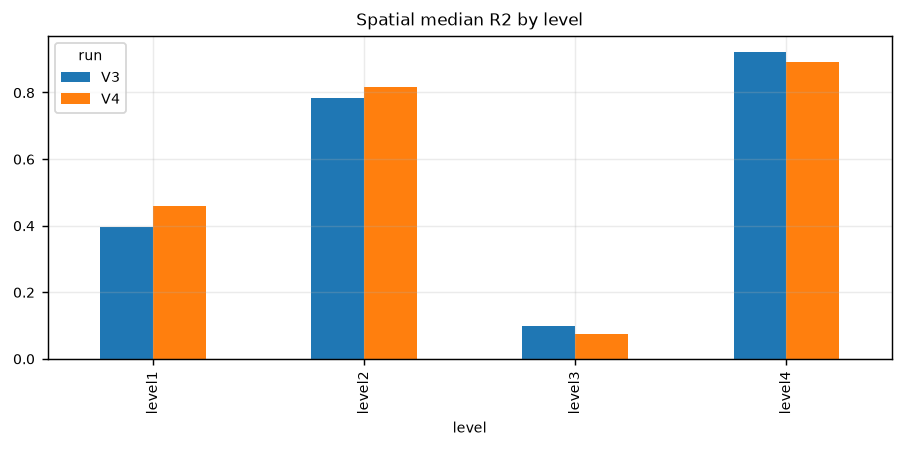
\includegraphics[width=.92\textwidth]{../figures/figure_01_spatial_r2.png}\caption{figure 01 spatial r2}\end{figure}
\begin{figure}[p]\centering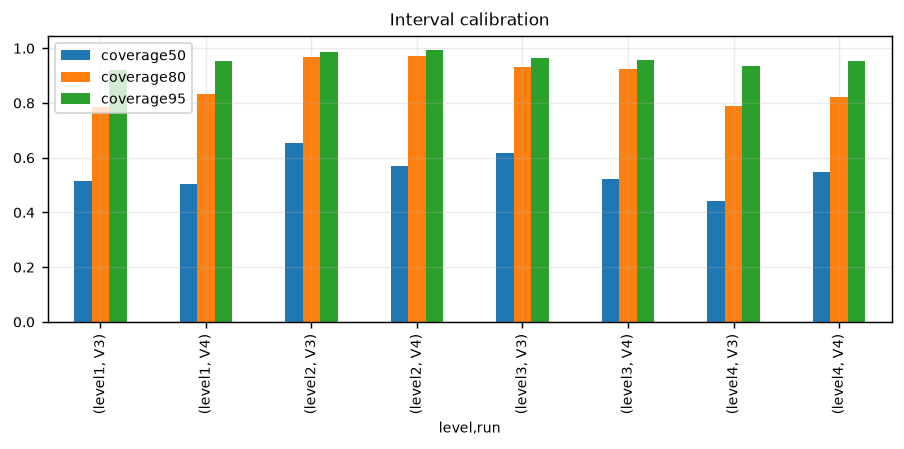
\includegraphics[width=.92\textwidth]{../figures/figure_02_calibration.png}\caption{figure 02 calibration}\end{figure}
\begin{figure}[p]\centering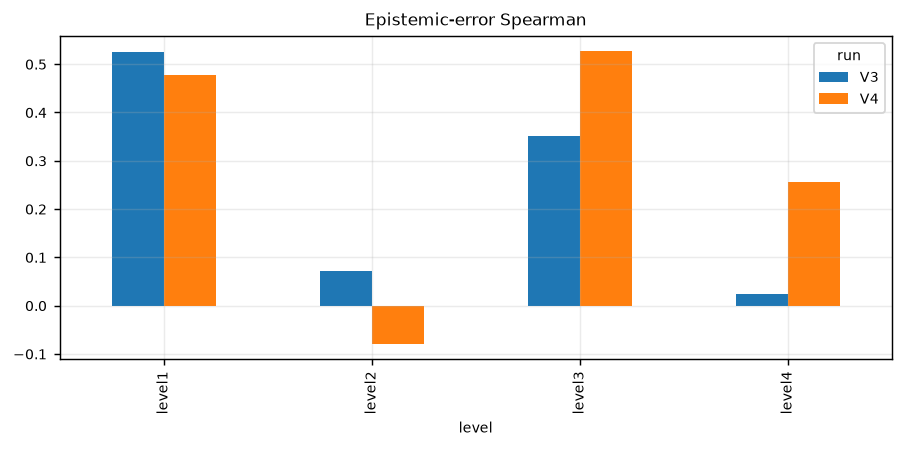
\includegraphics[width=.92\textwidth]{../figures/figure_03_uncertainty_error.png}\caption{figure 03 uncertainty error}\end{figure}
\begin{figure}[p]\centering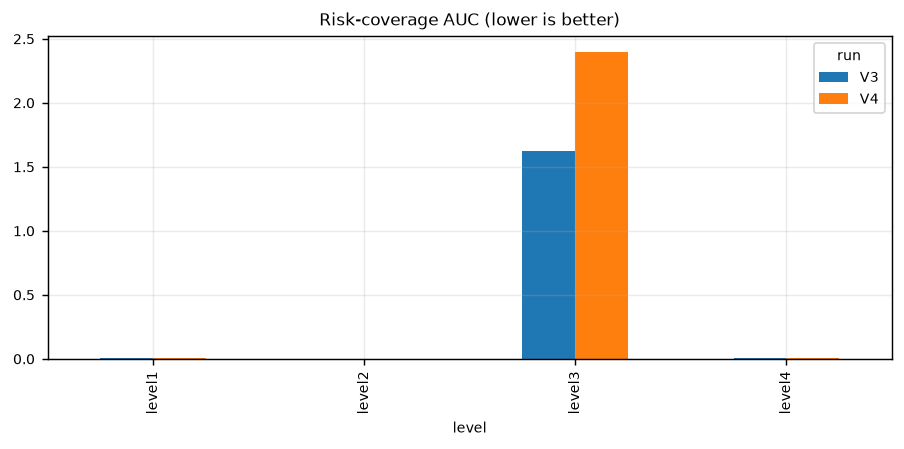
\includegraphics[width=.92\textwidth]{../figures/figure_04_risk_coverage.png}\caption{figure 04 risk coverage}\end{figure}
\begin{figure}[p]\centering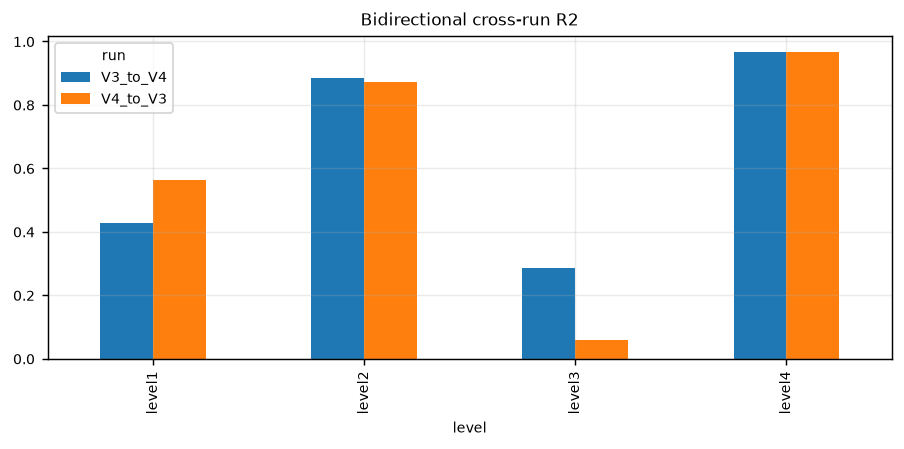
\includegraphics[width=.92\textwidth]{../figures/figure_05_cross_run.png}\caption{figure 05 cross run}\end{figure}
\begin{figure}[p]\centering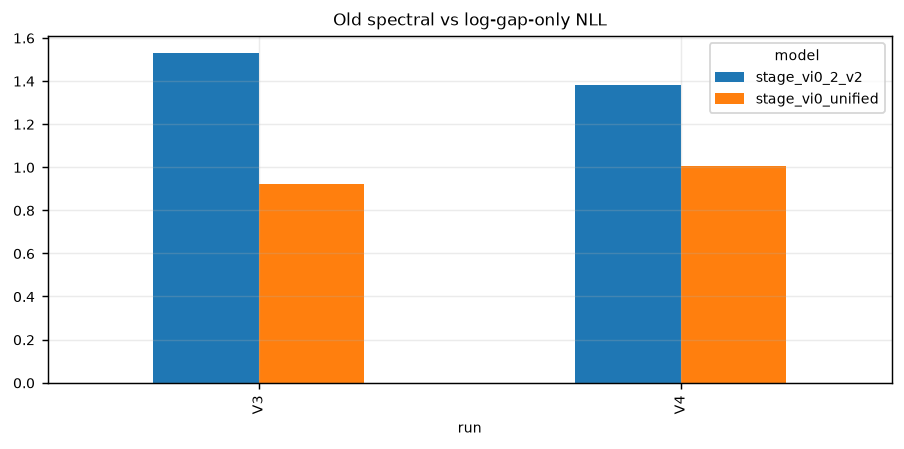
\includegraphics[width=.92\textwidth]{../figures/figure_06_spectral_comparison.png}\caption{figure 06 spectral comparison}\end{figure}
\begin{figure}[p]\centering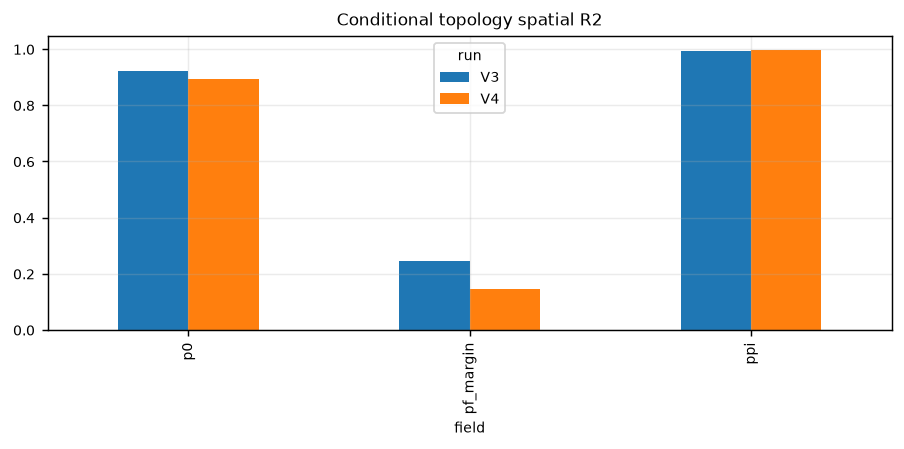
\includegraphics[width=.92\textwidth]{../figures/figure_07_topology_metrics.png}\caption{figure 07 topology metrics}\end{figure}
\begin{figure}[p]\centering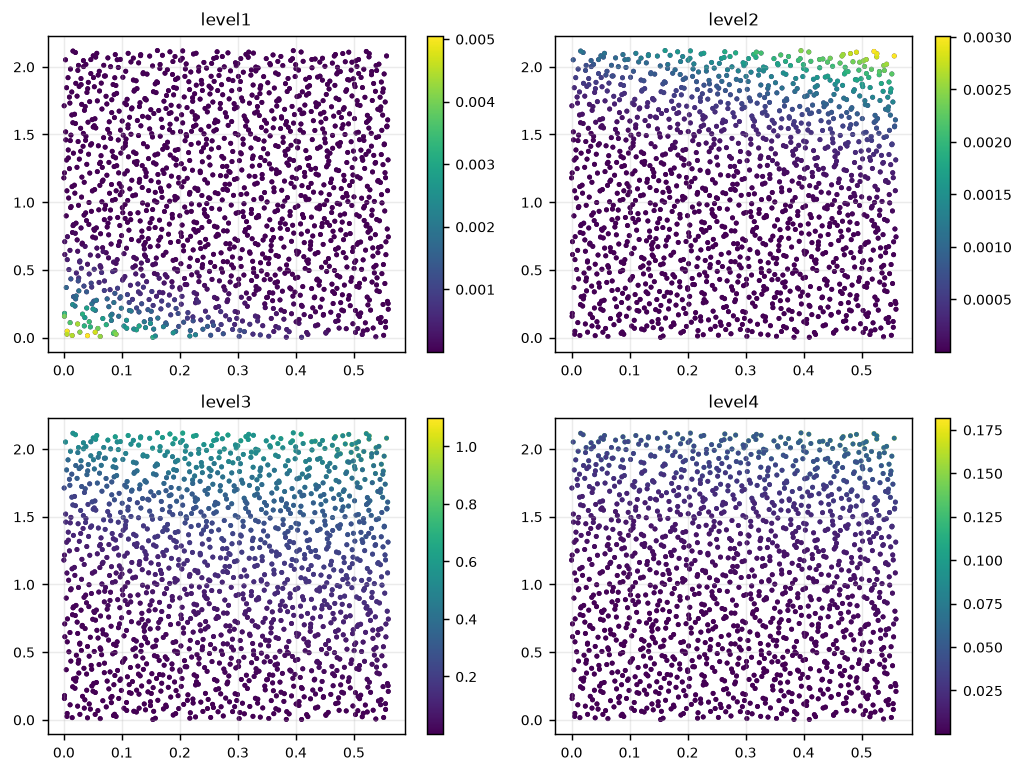
\includegraphics[width=.92\textwidth]{../figures/figure_08_probe_levels.png}\caption{figure 08 probe levels}\end{figure}
\begin{figure}[p]\centering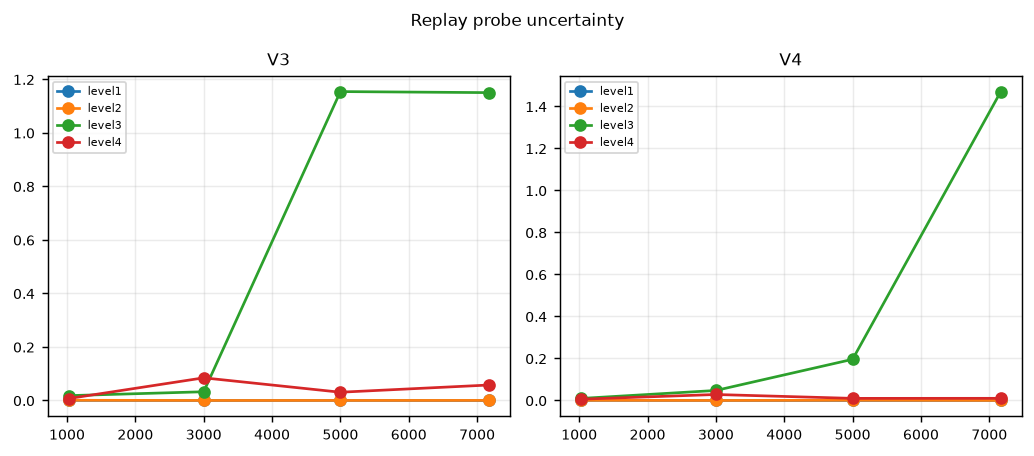
\includegraphics[width=.92\textwidth]{../figures/figure_09_replay_uncertainty.png}\caption{figure 09 replay uncertainty}\end{figure}
\begin{figure}[p]\centering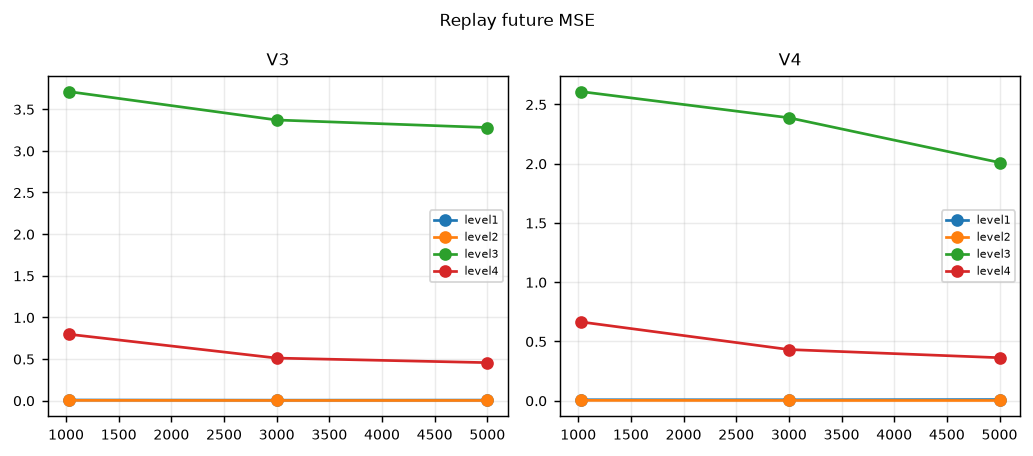
\includegraphics[width=.92\textwidth]{../figures/figure_10_replay_future.png}\caption{figure 10 replay future}\end{figure}
\begin{figure}[p]\centering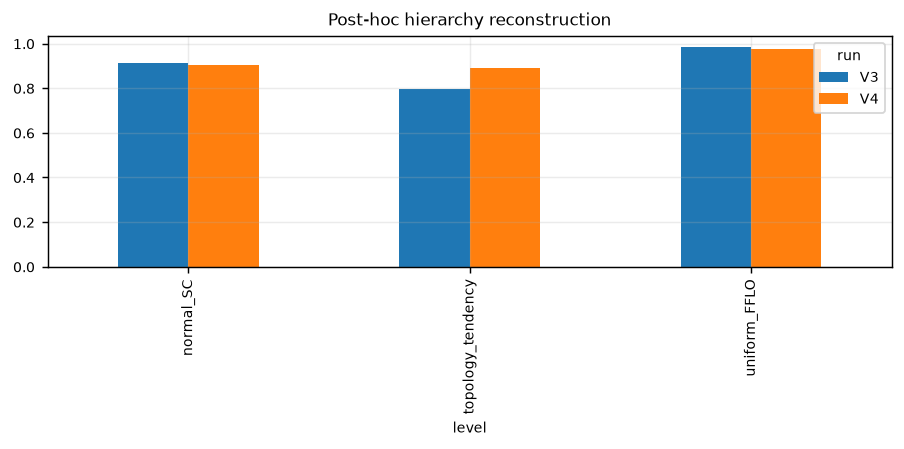
\includegraphics[width=.92\textwidth]{../figures/figure_11_phase_reconstruction.png}\caption{figure 11 phase reconstruction}\end{figure}
\begin{figure}[p]\centering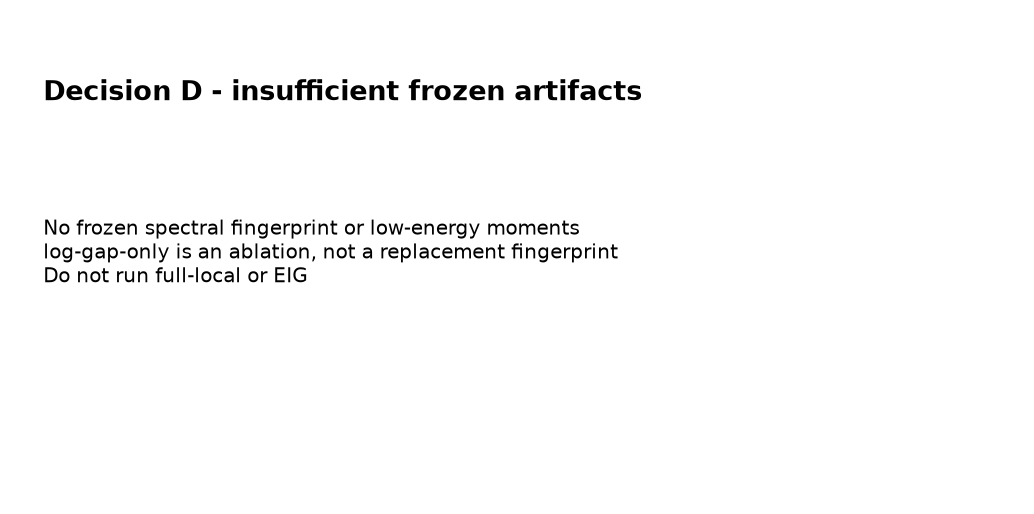
\includegraphics[width=.92\textwidth]{../figures/figure_12_decision.png}\caption{figure 12 decision}\end{figure}
\clearpage\section{Next artifact action}Export pre-existing fixed-grid spectra or physically defined low-energy moments if available. This report does not authorize exact calculations.\end{document}